\chapter{Dasar Teori}
\label{chap:Dasar Teori}

\section{jsoup}
\label{sec:jsoup}

\textit{Web scraping}\cite{Vargiu:2013} adalah teknik mendapatkan informasi dari sebuah situs \textit{web} secara otomatis. Dalam Java, \textit{web scraping} dapat diimplementasikan menggunakan \textit{library} jsoup\cite{jsoup}. API yang disediakan oleh jsoup dapat digunakan untuk mengekstrak dan memanipulasi data HTML. 

Subbab-subbab berikut menjelaskan kelas-kelas dari jsoup yang terkait dengan penelitian ini.

\subsection{Jsoup}

Kelas ini merupakan inti untuk mengakses fungsi jsoup. Salah satu \textit{method} yang dimiliki kelas ini adalah sebagai berikut:
\begin{itemize}
	\item \textbf{public static Connection connect(String url)} \\
		Berfungsi untuk membuat koneksi baru dengan suatu situs \textit{web}. \\
		\textbf{Parameter:}
		\begin{itemize}
			\item \textbf{url} URL situs \textit{web} dengan protokol HTTP atau HTTPS.
		\end{itemize}
		\textbf{Kembalian:} koneksi dengan situs \textit{web}.
\end{itemize}

\subsection{Connection}

Kelas ini merupakan interface yang menyediakan pengambilan data dari situs \textit{web}. Beberapa \textit{method} yang dimiliki kelas ini adalah sebagai berikut:

\begin{itemize}
	\item \textbf{Connection cookies(Map<String,String> cookies)} \\
		Berfungsi untuk menambahkan \textit{cookie}. \\
		\textbf{Parameter:}
		\begin{itemize}
			\item \textbf{cookies} \textit{map} dari \textit{cookie}.
		\end{itemize}
		\textbf{Kembalian:} koneksi dengan situs \textit{web}.
		
		\item \textbf{Connection data(String key, String value)} \\
		Berfungsi untuk menambahkan parameter data. \\
		\textbf{Parameter:}
		\begin{itemize}
			\item \textbf{key} kunci data.
			\item \textbf{value} nilai data.
		\end{itemize}
		\textbf{Kembalian:} koneksi dengan situs \textit{web}.
		
		\item \textbf{Connection method(Connection.Method method)} \\
		Berfungsi untuk mengatur metode pengiriman. \\
		\textbf{Parameter:}
		\begin{itemize}
			\item \textbf{method} metode pengiriman HTTP \textit{request}.
		\end{itemize}
		\textbf{Kembalian:} koneksi dengan situs \textit{web}.
		
		\item \textbf{Connection timeout(int millis)} \\
		Berfungsi untuk mengatur batas waktu \textit{request}. Batas waktu nol akan dianggap sebagai batas waktu yang tak terhingga. \\
		\textbf{Parameter:}
		\begin{itemize}
			\item \textbf{millis} banyaknya milisekon sebelum batas waktu.
		\end{itemize}
		\textbf{Kembalian:} koneksi dengan situs \textit{web}.
		
		\item \textbf{Connection validateTLSCertificates(boolean value)} \\
		Berfungsi untuk mengatur pemeriksaan sertifikat TLS untuk HTTPS \textit{request}. Nilai "`true"' untuk memeriksa dan nilai "`false"' untuk tidak memeriksa.\\
		\textbf{Parameter:}
		\begin{itemize}
			\item \textbf{value} status pemeriksaan sertifikat TLS.
		\end{itemize}
		\textbf{Kembalian:} koneksi dengan situs \textit{web}.
		
		\item \textbf{Connection.Response execute()} \\
		Berfungsi untuk mengirim \textit{request}.\\
		\textbf{Parameter:} tidak ada
		\textbf{Kembalian:} objek Response.	
\end{itemize}

\subsection{Response}

Kelas ini merepresentasikan HTTP \textit{response}. Response merupakan turunan dari kelas Base yang menangani response dan \textit{request}. Beberapa \textit{method} yang dimiliki kelas ini adalah sebagai berikut:
\begin{itemize}
	\item \textbf{Map<String,String> cookies()} \\
		\textit{Method} ini diturunkan dari kelas Base, berfungsi untuk mendapatkan seluruh \textit{cookies}. \\
		\textbf{Parameter:} tidak ada.
		\textbf{Kembalian:} seluruh \textit{cookies}.
		
		\item \textbf{Document parse()} \\
		Berfungsi untuk \textit{parsing} \textit{response body} menjadi dokumen. \\
		\textbf{Parameter:} tidak ada.
		\textbf{Kembalian:} koneksi dengan situs \textit{web}.
\end{itemize}


Response yang diperoleh akan di-\textit{parse} ke dalam bentuk \textit{Document Object Model} (DOM) yang direpresentasikan dalam kelas Document. Proses parsing dapat dilakukan dengan pemanggilan method parse() oleh objek Response. Document yang telah diperoleh dari hasil parsing dapat diseleksi untuk mendapatkan data yang diinginkan. Dalam menyeleksi Document, jsoup memanfaatkan CSS \textit{Selector} untuk mendapatkan elemen HTML yang dipanggil oleh objek Document dengan method select(). Hasil proses seleksi akan ditampung ke dalam objek bertipe Elements yang merepresentasikan elemen-elemen pada HTML. 

\section{Chrome DevTools}
\label{sec:devtools}

Chrome Developer Tools (DevTools) \cite{devtools} adalah perangkat \textit{debugging} yang dimiliki Google Chrome. Saat menunjungi suatu website, pengguna DevTools dapat melakukan debugging pada website tersebut. DevTools dapat diakses dengan menekan "`Ctrl+Shift+I"' saat sedang membuka suatu website.  

Fitur-fitur yang dimiliki DevTools antara lain:
\begin{enumerate}
	\item \textit{Elements}, memeriksa dan mengubah elemen HTML dan \textit{style} dari suatu \textit{website}.
	\item \textit{Console}, mendapatkan informasi pengembangan dan berinteraksi dengan dokumen.
	\item \textit{Sources}, melakukan \textit{debugging} pada JavaScript dengan menentukan \textit{breakpoint}.
	\item \textit{Network}, memantau kinerja jaringan pada \textit{website} secara \textit{real-time}.
	\item \textit{Audits}, menganalisa halaman yang dimuat.
	\item \textit{Timeline}, menampilkan alur waktu saat memuat halaman.
	\item \textit{Profiles}, menggambarkan waktu eksekusi dan penggunaan memori saat memuat halaman.
	\item \textit{Resources}, memeriksa sumber daya halaman yang dapat berupa basis data, \textit{cookies}, dan \textit{cache}.
\end{enumerate}

\begin{figure}[H]
	\centering
	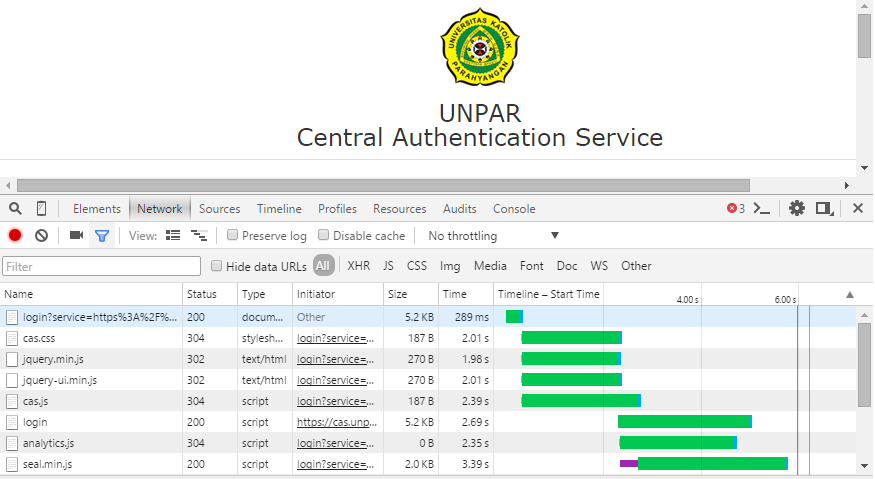
\includegraphics[scale=0.5]{Gambar/chrome-devtools}
	\caption{Chrome DevTools} 
	\label{fig:chrome_devtools}
\end{figure}



\section{Play Framework}
\label{sec:play}

Play Framework \cite{Leroux:2014} merupakan sebuah web framework berbasis Java dan Scala. Play juga menggunakan \textit{design pattern} Model-View-Controller (MVC) di mana \textit{model} dan \textit{controller} menggunakan Java sedangkan \textit{view} menggunakan Scala dan HTML. 
